% Options for packages loaded elsewhere
\PassOptionsToPackage{unicode}{hyperref}
\PassOptionsToPackage{hyphens}{url}
\documentclass[
  ignorenonframetext,
]{beamer}
\newif\ifbibliography
\usepackage{pgfpages}
\setbeamertemplate{caption}[numbered]
\setbeamertemplate{caption label separator}{: }
\setbeamercolor{caption name}{fg=normal text.fg}
\beamertemplatenavigationsymbolsempty
% remove section numbering
\setbeamertemplate{part page}{
  \centering
  \begin{beamercolorbox}[sep=16pt,center]{part title}
    \usebeamerfont{part title}\insertpart\par
  \end{beamercolorbox}
}
\setbeamertemplate{section page}{
  \centering
  \begin{beamercolorbox}[sep=12pt,center]{section title}
    \usebeamerfont{section title}\insertsection\par
  \end{beamercolorbox}
}
\setbeamertemplate{subsection page}{
  \centering
  \begin{beamercolorbox}[sep=8pt,center]{subsection title}
    \usebeamerfont{subsection title}\insertsubsection\par
  \end{beamercolorbox}
}
% Prevent slide breaks in the middle of a paragraph
\widowpenalties 1 10000
\raggedbottom
\AtBeginPart{
  \frame{\partpage}
}
\AtBeginSection{
  \ifbibliography
  \else
    \frame{\sectionpage}
  \fi
}
\AtBeginSubsection{
  \frame{\subsectionpage}
}
\usepackage{iftex}
\ifPDFTeX
  \usepackage[T1]{fontenc}
  \usepackage[utf8]{inputenc}
  \usepackage{textcomp} % provide euro and other symbols
\else % if luatex or xetex
  \usepackage{unicode-math} % this also loads fontspec
  \defaultfontfeatures{Scale=MatchLowercase}
  \defaultfontfeatures[\rmfamily]{Ligatures=TeX,Scale=1}
\fi
\usepackage{lmodern}
\ifPDFTeX\else
  % xetex/luatex font selection
\fi
% Use upquote if available, for straight quotes in verbatim environments
\IfFileExists{upquote.sty}{\usepackage{upquote}}{}
\IfFileExists{microtype.sty}{% use microtype if available
  \usepackage[]{microtype}
  \UseMicrotypeSet[protrusion]{basicmath} % disable protrusion for tt fonts
}{}
\makeatletter
\@ifundefined{KOMAClassName}{% if non-KOMA class
  \IfFileExists{parskip.sty}{%
    \usepackage{parskip}
  }{% else
    \setlength{\parindent}{0pt}
    \setlength{\parskip}{6pt plus 2pt minus 1pt}}
}{% if KOMA class
  \KOMAoptions{parskip=half}}
\makeatother
\usepackage{color}
\usepackage{fancyvrb}
\newcommand{\VerbBar}{|}
\newcommand{\VERB}{\Verb[commandchars=\\\{\}]}
\DefineVerbatimEnvironment{Highlighting}{Verbatim}{commandchars=\\\{\}}
% Add ',fontsize=\small' for more characters per line
\newenvironment{Shaded}{}{}
\newcommand{\AlertTok}[1]{\textcolor[rgb]{1.00,0.00,0.00}{\textbf{#1}}}
\newcommand{\AnnotationTok}[1]{\textcolor[rgb]{0.38,0.63,0.69}{\textbf{\textit{#1}}}}
\newcommand{\AttributeTok}[1]{\textcolor[rgb]{0.49,0.56,0.16}{#1}}
\newcommand{\BaseNTok}[1]{\textcolor[rgb]{0.25,0.63,0.44}{#1}}
\newcommand{\BuiltInTok}[1]{\textcolor[rgb]{0.00,0.50,0.00}{#1}}
\newcommand{\CharTok}[1]{\textcolor[rgb]{0.25,0.44,0.63}{#1}}
\newcommand{\CommentTok}[1]{\textcolor[rgb]{0.38,0.63,0.69}{\textit{#1}}}
\newcommand{\CommentVarTok}[1]{\textcolor[rgb]{0.38,0.63,0.69}{\textbf{\textit{#1}}}}
\newcommand{\ConstantTok}[1]{\textcolor[rgb]{0.53,0.00,0.00}{#1}}
\newcommand{\ControlFlowTok}[1]{\textcolor[rgb]{0.00,0.44,0.13}{\textbf{#1}}}
\newcommand{\DataTypeTok}[1]{\textcolor[rgb]{0.56,0.13,0.00}{#1}}
\newcommand{\DecValTok}[1]{\textcolor[rgb]{0.25,0.63,0.44}{#1}}
\newcommand{\DocumentationTok}[1]{\textcolor[rgb]{0.73,0.13,0.13}{\textit{#1}}}
\newcommand{\ErrorTok}[1]{\textcolor[rgb]{1.00,0.00,0.00}{\textbf{#1}}}
\newcommand{\ExtensionTok}[1]{#1}
\newcommand{\FloatTok}[1]{\textcolor[rgb]{0.25,0.63,0.44}{#1}}
\newcommand{\FunctionTok}[1]{\textcolor[rgb]{0.02,0.16,0.49}{#1}}
\newcommand{\ImportTok}[1]{\textcolor[rgb]{0.00,0.50,0.00}{\textbf{#1}}}
\newcommand{\InformationTok}[1]{\textcolor[rgb]{0.38,0.63,0.69}{\textbf{\textit{#1}}}}
\newcommand{\KeywordTok}[1]{\textcolor[rgb]{0.00,0.44,0.13}{\textbf{#1}}}
\newcommand{\NormalTok}[1]{#1}
\newcommand{\OperatorTok}[1]{\textcolor[rgb]{0.40,0.40,0.40}{#1}}
\newcommand{\OtherTok}[1]{\textcolor[rgb]{0.00,0.44,0.13}{#1}}
\newcommand{\PreprocessorTok}[1]{\textcolor[rgb]{0.74,0.48,0.00}{#1}}
\newcommand{\RegionMarkerTok}[1]{#1}
\newcommand{\SpecialCharTok}[1]{\textcolor[rgb]{0.25,0.44,0.63}{#1}}
\newcommand{\SpecialStringTok}[1]{\textcolor[rgb]{0.73,0.40,0.53}{#1}}
\newcommand{\StringTok}[1]{\textcolor[rgb]{0.25,0.44,0.63}{#1}}
\newcommand{\VariableTok}[1]{\textcolor[rgb]{0.10,0.09,0.49}{#1}}
\newcommand{\VerbatimStringTok}[1]{\textcolor[rgb]{0.25,0.44,0.63}{#1}}
\newcommand{\WarningTok}[1]{\textcolor[rgb]{0.38,0.63,0.69}{\textbf{\textit{#1}}}}
\usepackage{graphicx}
\makeatletter
\newsavebox\pandoc@box
\newcommand*\pandocbounded[1]{% scales image to fit in text height/width
  \sbox\pandoc@box{#1}%
  \Gscale@div\@tempa{\textheight}{\dimexpr\ht\pandoc@box+\dp\pandoc@box\relax}%
  \Gscale@div\@tempb{\linewidth}{\wd\pandoc@box}%
  \ifdim\@tempb\p@<\@tempa\p@\let\@tempa\@tempb\fi% select the smaller of both
  \ifdim\@tempa\p@<\p@\scalebox{\@tempa}{\usebox\pandoc@box}%
  \else\usebox{\pandoc@box}%
  \fi%
}
% Set default figure placement to htbp
\def\fps@figure{htbp}
\makeatother
\setlength{\emergencystretch}{3em} % prevent overfull lines
\providecommand{\tightlist}{%
  \setlength{\itemsep}{0pt}\setlength{\parskip}{0pt}}
% Slide layout defaults for warning-clean scientific decks.
\usepackage{etoolbox}
\IfFileExists{xurl.sty}{\usepackage{xurl}}{}
\IfFileExists{seqsplit.sty}{\usepackage{seqsplit}}{\newcommand{\seqsplit}[1]{#1}}
\protected\def\breakseq#1{\seqsplit{#1}}
\protected\def\breaktt#1{\begingroup\ttfamily\seqsplit{#1}\endgroup}
\setlength{\emergencystretch}{6em}
\tolerance=5000
\hbadness=10000
\hfuzz=1pt
\setlength{\tabcolsep}{2pt}
\AtBeginEnvironment{longtable}{\tiny\renewcommand{\arraystretch}{0.86}\setlength{\tabcolsep}{1pt}}
\AtBeginEnvironment{tabular}{\tiny\renewcommand{\arraystretch}{0.86}\setlength{\tabcolsep}{1pt}}

% Natbib and cross-reference fallbacks — slides don't load natbib
% or cleveref, but combined-PDF manuscript prose may emit these
% commands. The fallback renders citations as a bracketed key list
% and cross-references as detokenized labels so slides don't fail on
% undefined control sequences or raw underscores. \providecommand is
% a no-op if packages load later.
\providecommand{\citep}[1]{[#1]}
\providecommand{\citet}[1]{#1}
\providecommand{\citealp}[1]{#1}
\providecommand{\citeauthor}[1]{#1}
\providecommand{\citeyear}[1]{#1}
\providecommand{\cref}[1]{\texttt{\detokenize{#1}}}
\providecommand{\Cref}[1]{\texttt{\detokenize{#1}}}

\newtheorem{proposition}{Proposition}
\newtheorem{hypothesis}{Hypothesis}
\usepackage{bookmark}
\IfFileExists{xurl.sty}{\usepackage{xurl}}{} % add URL line breaks if available
\urlstyle{same}
% fallback for those not using the hyperref driver hyperxmp:
\makeatletter
\@ifundefined{xmpquote}{\newcommand{\xmpquote}[1]{#1}}{}
\makeatother
\hypersetup{
  hidelinks,
  pdfcreator={LaTeX via pandoc}}

\author{\texorpdfstring{}{}}
\date{}

\begin{document}

\section{Pools: Fonds as Passive Data Resources}\label{sec:pools}

\begin{frame}[fragile,allowframebreaks]{What Is a Fond?}
\protect\phantomsection\label{what-is-a-fond}
A \textbf{fond} is a versioned, read-only data pool that any project in
the repository can consume without modifying. The term evokes the
culinary concept of a concentrated stock --- a stable base that enriches
whatever is built on top of it. Fonds live under the top-level
\texttt{fonds/\textless{}scope\textgreater{}/\textless{}name\textgreater{}/}
directory, each containing a manifest file (\texttt{fonds.yaml}), a
\texttt{data/} subdirectory, and optional documentation. This
architecture separates \emph{data ownership} from \emph{data usage}:
research projects in \texttt{projects/} are consumers, not producers, of
fond data. The separation prevents the accretion of project-specific
mutations in shared resources --- a recurring source of reproducibility
failures in collaborative research software \breakseq{[@Wilson2014best]}.

The three-layer taxonomy (bibliography, contacts, datasets) maps to the
three most common categories of curated research data: citable
literature, human collaboration networks, and input/output datasets.
Each category carries its own schema enforced by
\breaktt{rules/templates/template\_manuscript\_rules}. @fig:taxonomy
compares the three fond types field-by-field: every fond shares a
manifest and a \texttt{type} discriminator, but the source-of-truth
format, secondary mirror, and deduplication key differ by category --- a
consequence of each category's data having a naturally different
canonical representation (BibTeX for citations, YAML for structured
contact records, YAML for dataset metadata).

\begin{figure}
\centering
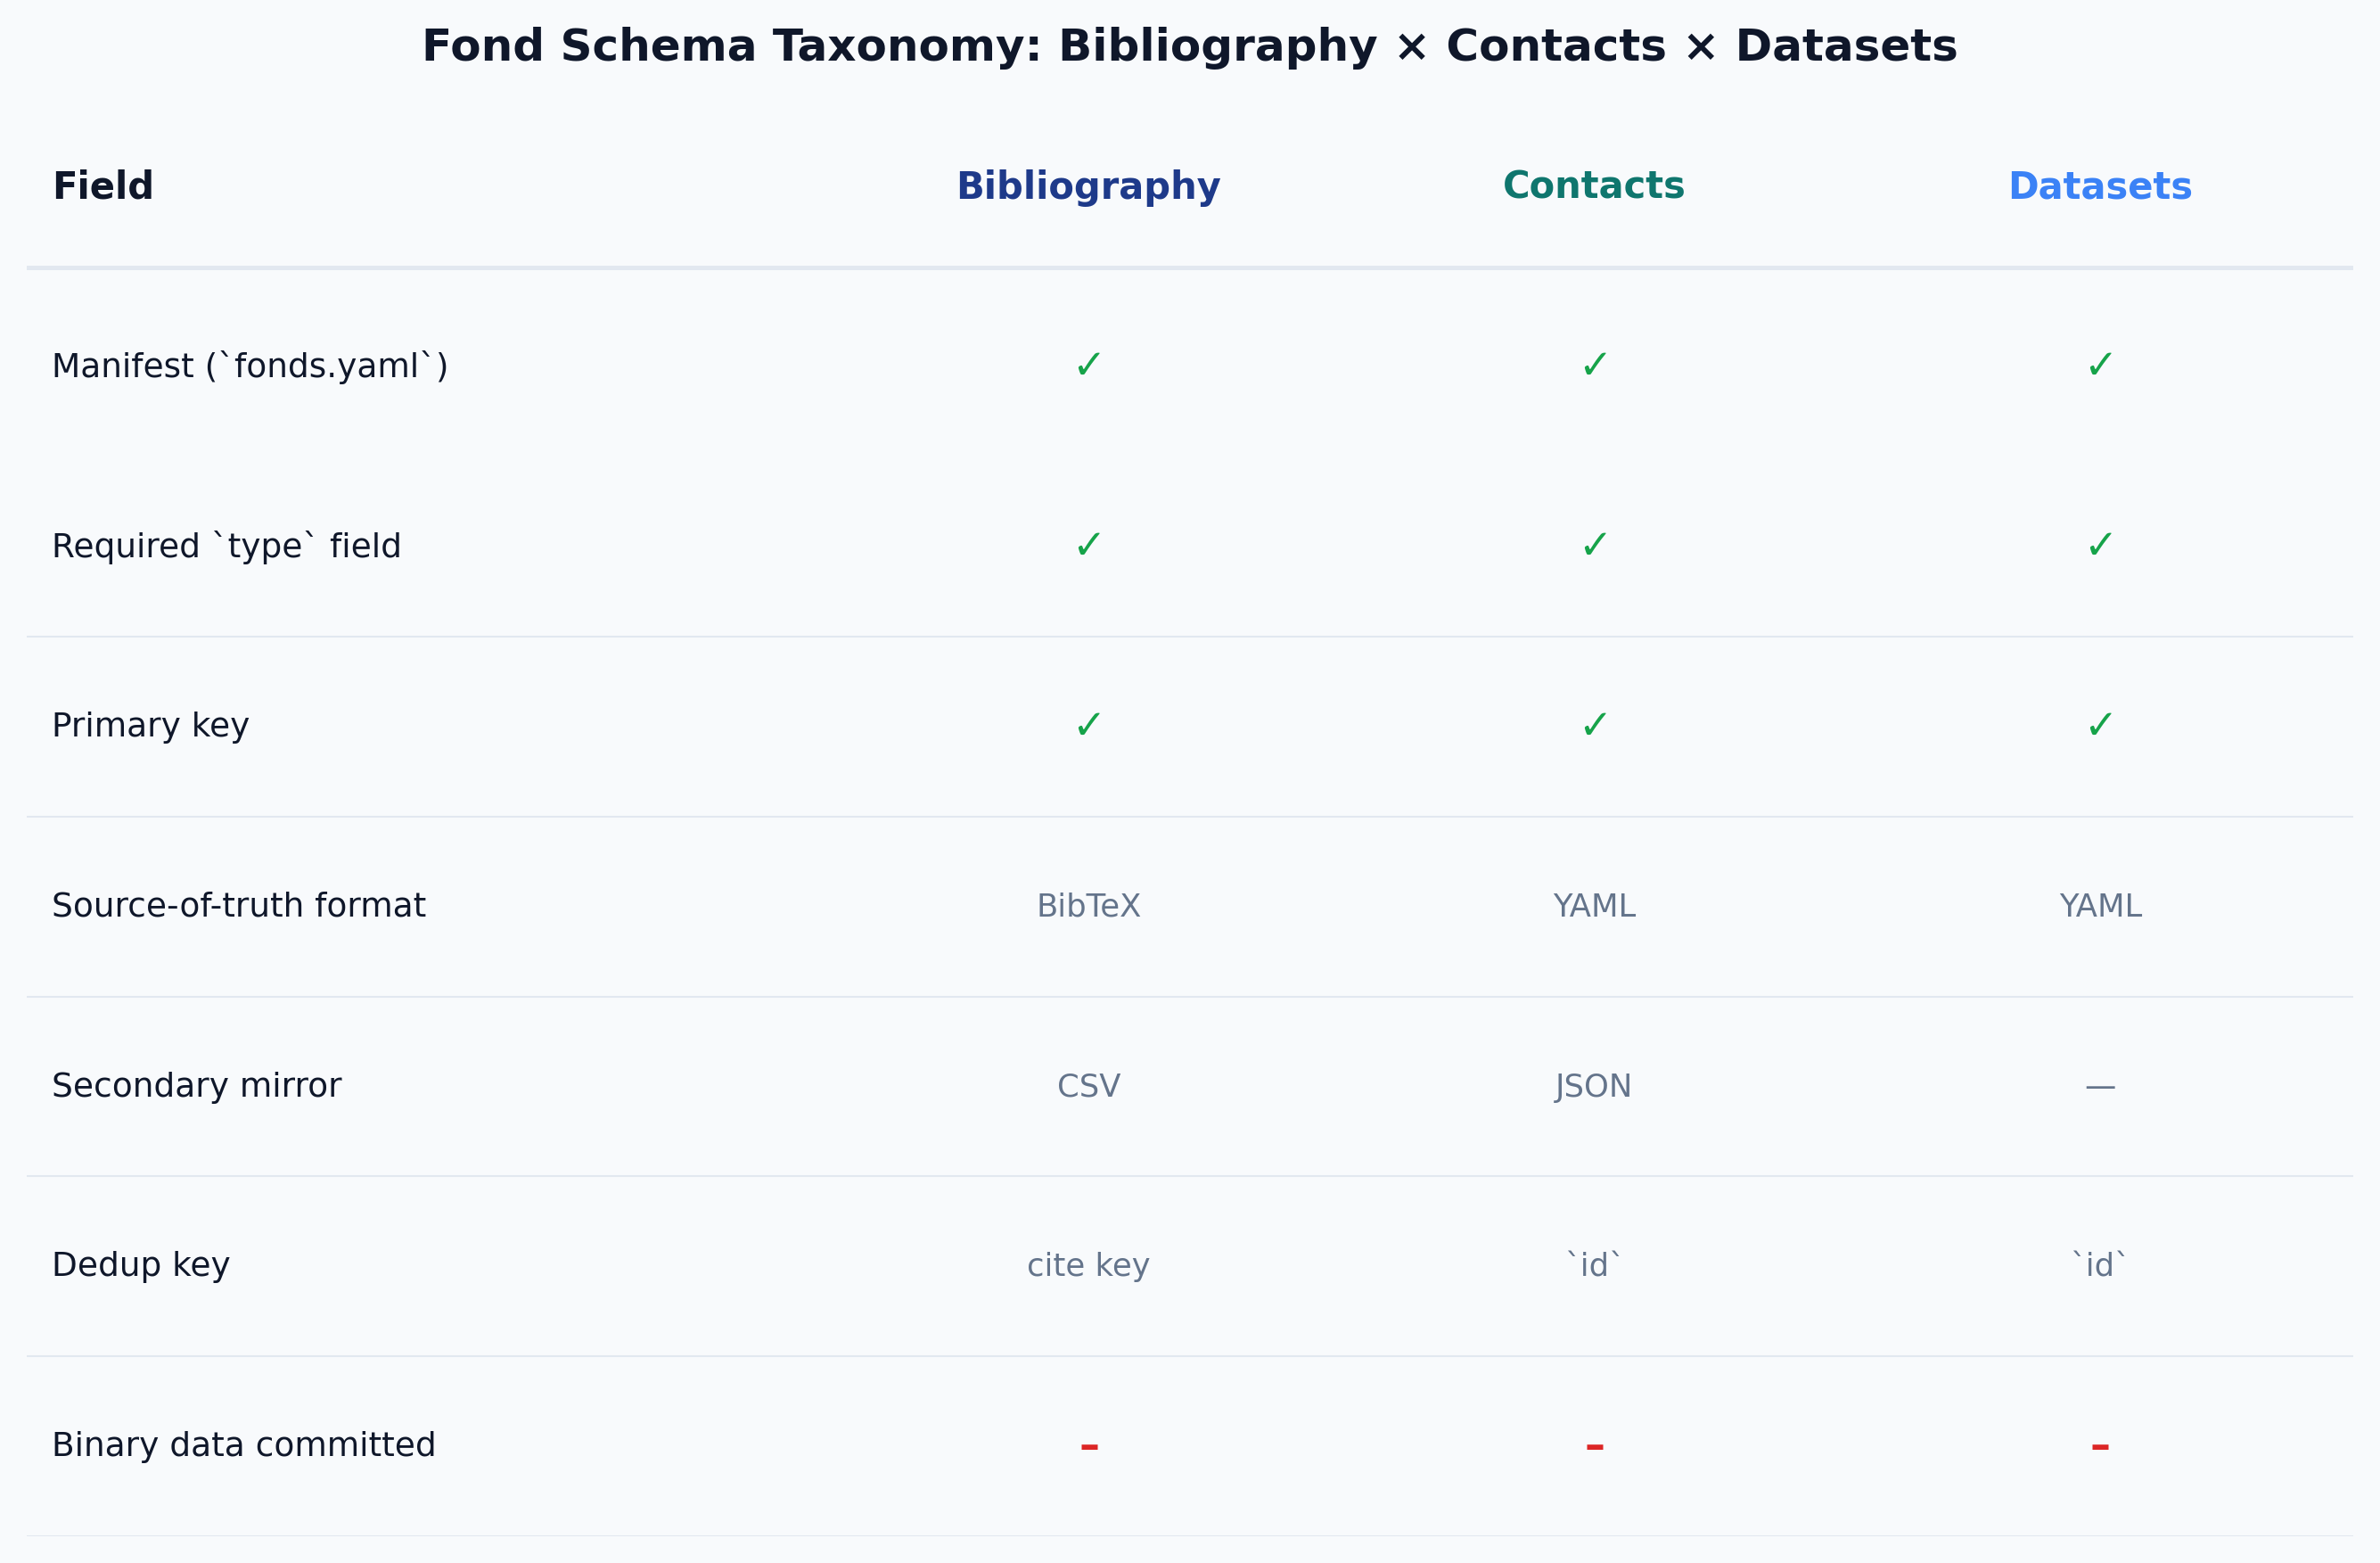
\includegraphics[width=0.85\linewidth,height=0.46\textheight,keepaspectratio,alt={Schema taxonomy comparison across the three fond types. Each fond declares a manifest and a type field; source-of-truth format, secondary mirror, and dedup key differ by category.}]{../figures/fond_taxonomy.png}
\caption{Schema taxonomy comparison across the three fond types. Each
fond declares a manifest and a \protect\texttt{type} field;
source-of-truth format, secondary mirror, and dedup key differ by
category.}\label{fig:taxonomy}
\end{figure}
\end{frame}

\begin{frame}[fragile,allowframebreaks]{The Three Template Fonds}
\protect\phantomsection\label{the-three-template-fonds}
\begin{block}{\breaktt{template\_bibliography}}
\protect\phantomsection\label{template_bibliography}
The \breaktt{template\_bibliography} fond is a curated reference library
stored in two formats: a BibTeX file (\breaktt{data/references.bib}) as
source of truth, and a flat CSV export (\breaktt{data/references.csv})
for programmatic querying. Deduplication is enforced on the cite key
(the primary CSV column). The collection spans foundational
machine-learning works --- the transformer architecture
\breakseq{[@Vaswani2017attention]}, early convolutional network research
\breakseq{[@LeCun1998gradient]}, and large-scale language model pre-training
\breakseq{[@Brown2020gpt3]} --- alongside software-engineering references on
best practices \breakseq{[@Wilson2014best]} and robust software design
\breakseq{[@Taschuk2017ten]}. In the current integration run, the fond contains
\textbf{8 entries}.

The bibliography fond illustrates the \emph{registry pattern}
\breakseq{[@Fowler2002patterns]}: a single authoritative list is maintained
centrally, and all projects reference it rather than keeping private
copies. This guarantees citation consistency across all exemplar
manuscripts.
\end{block}

\begin{block}{\breaktt{template\_contacts}}
\protect\phantomsection\label{template_contacts}
The \breaktt{template\_contacts} fond holds a registry of research
collaborators, advisors, and reviewers. Each entry is a YAML object with
required fields \texttt{id} (a unique slug), \texttt{name}, and
\texttt{email}, plus optional fields \texttt{affiliation},
\texttt{role}, \texttt{orcid}, \texttt{website}, and \texttt{notes}. The
YAML file (\breaktt{data/contacts.yaml}) is the source of truth; a JSON
mirror (\breaktt{data/contacts.json}) supports consumers that prefer JSON
deserialization. Deduplication is enforced on the \texttt{id} field at
validation time.
\end{block}

\begin{block}{\breaktt{template\_datasets}}
\protect\phantomsection\label{template_datasets}
The \breaktt{template\_datasets} fond catalogs dataset metadata:
provenance, licensing, format, size, access URLs, and research tasks. It
intentionally stores \emph{metadata only} --- no actual data binaries
are committed to the repository. This design aligns with the principle
that version control systems should track configuration and metadata
rather than large binary artefacts \breakseq{[@Kluyver2016jupyter]}. Dataset
entries require \texttt{id}, \texttt{name}, \texttt{version}, and
\texttt{license} fields. Exemplar entries reference classic benchmarks
such as MNIST (introduced in \breakseq{[@LeCun1998gradient]}) and large-scale
corpora used in language-model research \breakseq{[@Brown2020gpt3]}.
\end{block}
\end{frame}

\begin{frame}[fragile,allowframebreaks]{The \texttt{fonds.yaml}
Manifest}
\protect\phantomsection\label{the-fonds.yaml-manifest}
Every fond root must contain a \texttt{fonds.yaml} manifest with at
minimum three fields:

\begin{Shaded}
\begin{Highlighting}[]
\FunctionTok{type}\KeywordTok{:}\AttributeTok{ bibliography}\CommentTok{   \# bibliography | contacts | datasets}
\FunctionTok{description}\KeywordTok{:}\AttributeTok{ }\StringTok{"Human{-}readable description of the fond"}
\FunctionTok{version}\KeywordTok{:}\AttributeTok{ }\StringTok{"1.0"}
\FunctionTok{tags}\KeywordTok{:}\AttributeTok{ }\KeywordTok{[}\AttributeTok{curated}\KeywordTok{,}\AttributeTok{ exemplar}\KeywordTok{]}
\end{Highlighting}
\end{Shaded}

The \texttt{type} field governs which reader function is appropriate and
what schema the \texttt{data/} directory is expected to follow. The
\texttt{version} field is incremented whenever the schema changes,
enabling consumers to detect and handle schema drift without silent
failures.
\end{frame}

\begin{frame}[fragile,allowframebreaks]{The \texttt{fonds\_reader}
Module}
\protect\phantomsection\label{the-fonds_reader-module}
The \breaktt{src/fonds\_reader.py} module provides three reader functions
--- one per fond type --- plus a convenience aggregator:

\begin{Shaded}
\begin{Highlighting}[]
\ImportTok{from}\NormalTok{ src.fonds\_reader }\ImportTok{import}\NormalTok{ (}
\NormalTok{    read\_bibliography\_fond,}
\NormalTok{    read\_contacts\_fond,}
\NormalTok{    read\_datasets\_fond,}
\NormalTok{    read\_all\_fonds,}
\NormalTok{)}

\NormalTok{bib      }\OperatorTok{=}\NormalTok{ read\_bibliography\_fond()   }\CommentTok{\# dict | None}
\NormalTok{contacts }\OperatorTok{=}\NormalTok{ read\_contacts\_fond()       }\CommentTok{\# dict | None}
\NormalTok{datasets }\OperatorTok{=}\NormalTok{ read\_datasets\_fond()       }\CommentTok{\# dict | None}
\NormalTok{all\_fonds }\OperatorTok{=}\NormalTok{ read\_all\_fonds()          }\CommentTok{\# \{"bibliography": ..., "contacts": ..., "datasets": ...\}}
\end{Highlighting}
\end{Shaded}

Each reader resolves the repository root from
\texttt{pathlib.Path(\_\_file\_\_).resolve().parents{[}4{]}}, checks
that the manifest and data files exist before touching them, and wraps
the actual YAML parse in a
\breaktt{try/except\ (OSError,\ UnicodeDecodeError,\ yaml.YAMLError)}
block. A missing path or a malformed file both degrade the same way ---
a logged warning and a \texttt{None} return --- so the integration
pipeline keeps going when a fond has not yet been populated by a
parallel agent \breakseq{[@Taschuk2017ten]}. In the current run, 3 of 3
expected fonds were successfully loaded (see @fig:counts).
\end{frame}

\begin{frame}[allowframebreaks]{Resilience by Design}
\protect\phantomsection\label{resilience-by-design}
The fond layer enforces resilience at two levels. At the
\textbf{structural} level, readers tolerate missing fonds entirely. At
the \textbf{schema} level, the manifest version field allows consumers
to check compatibility before processing data. This two-level approach
means a fond can evolve its schema without breaking existing consumers
that have not yet been updated: the consumer detects the version
mismatch and either adapts to it or skips the fond outright, instead of
crashing on data it doesn't recognise.
\end{frame}

\begin{frame}[fragile,allowframebreaks]{Worked Example: Graceful
Degradation in Practice}
\protect\phantomsection\label{worked-example-graceful-degradation-in-practice}
Consider a concrete failure scenario: a parallel automation agent is in
the process of authoring \breaktt{fonds/templates/template\_contacts/}
and has written \texttt{fonds.yaml} but not yet populated
\breaktt{data/contacts.yaml}. A naive reader would raise
\breaktt{FileNotFoundError} the instant \breaktt{read\_contacts\_fond()}
is called, aborting the entire integration pipeline over one incomplete
resource. \breaktt{read\_contacts\_fond()} instead:

\begin{enumerate}
\tightlist
\item
  Resolves the repository root via
  \texttt{pathlib.Path(\_\_file\_\_).resolve().parents{[}4{]}}.
\item
  Checks \breaktt{manifest\_path.exists()} and
  \breaktt{contacts\_path.exists()} explicitly before any read; on a
  missing path, logs
  \breaktt{logger.warning("contacts\ fond:\ missing\ \%s",\ p)} and
  returns \texttt{None} immediately --- no exception is ever raised for
  the common case of an in-progress resource.
\item
  If both paths exist, parses each with \breaktt{yaml.safe\_load()}
  inside a
  \breaktt{try/except\ (OSError,\ UnicodeDecodeError,\ yaml.YAMLError)}
  block, so a present-but-malformed file degrades the same way as a
  missing one.
\item
  \breaktt{run\_integration\_demo()} records the reduced count in the
  summary dict rather than propagating any exception.
\item
  The manuscript token \texttt{3} reflects the reduced count honestly
  --- the pipeline never claims a fond loaded that did not.
\end{enumerate}

This sequence is exercised directly by
\breaktt{tests/test\_fonds\_reader.py::test\_missing\_data\_dir\_contacts\_returns\_none},
which constructs a fond directory with a manifest but no \texttt{data/}
subdirectory and asserts the reader returns \texttt{None} rather than
raising. The same existence-check-then-parse pattern repeats identically
across \texttt{fonds\_reader.py}'s three readers,
\breaktt{rules\_applier.py}, and \breaktt{tools\_invoker.py}, which is why
@fig:resilience presents it as one repeated design, not three
independent ad-hoc fixes.
\end{frame}

\end{document}
